\section{Zielsetzung}
\label{sec:Zielsetzung}

Ziel des Versuches ist es, die Magnetfelder
verschiedener Spulen nachvollziehen zu können
und die Hysteresekurve eines Ferromagneten zu
nutzen um seine Remanenz und Koerzität zu
bestimmen.

\section{Theorie}
\label{sec:Theorie}

\subsection{Spulen}

Magnetfelder entstehen durch das bewegen elektrischer Ladungen.
Daher erzeugt auch jeder stromdurchflossene Leiter ein magnetisches
Feld. Das Biot-Savartsche Gesetz gibt dabei den magnetischen Fluss
$\symbf{B}$ an einem Punkt $\symbf{r}$ mit dem Abstand $r=|\symbf{r}|$
von einem mit dem Strom $I$ durchflossenen leiter an:

\begin{equation}
  \symup{d}\,B=\frac{\mu_0I}{4\pi}\frac{\symup{d}\,\symbf{s}\times\symbf{r}}{r^3}
  \label{eqn:bs}
\end{equation}

\begin{figure}
  \centering
  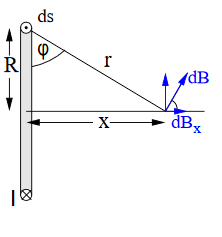
\includegraphics[width=0.5\textwidth]{content/images/biotsavartidee.png}
  \caption{Veranschaulichung des Biot-Savart Gesetzes an einer Leiterwindung\cite{anleitung}.}
  \label{fig:bs}
\end{figure}

Für eine vollständige Windung eines Leiters ergibt sich
durch integrieren über \eqref{eqn:bs} folgende Gleichung:

\begin{equation}
  \symbf{B}(x)=\frac{\mu_0I}{2}\frac{R^2}{\left(R^2+x^2\right)^{3/2}}\cdot \symbf{e}_x
  \label{eqn:bswdg}
\end{equation}

welchen in Abb. \ref{fig:bs} noch einmal veranschaulicht ist.
Für eine Spule mit $n$ Windungen wird dieser Wert ver-$n$-facht.
In einer langen Spule ist der magnetische Fluss in der Mitte ungefähr
konstant und zeigt in Richtung der Längsachse der Spule.

Es ergibt sich betragsmäßig ungefähr:
\begin{equation}
  B = \mu_{\symup{r}}\mu_0\frac{n}{l}I
  \label{eqn:Bspule}
\end{equation}

Formt man aus dieser Spule einen Torus mit Radius $r_{\symup{T}}$
so ergibt sich dafür
\begin{equation}
  B = \mu_{\symup{r}}\mu_0\frac{n}{2\pi r_{\symup{T}}}I
  \label{eqn:Btorus}
\end{equation}

Um ein möglichst homogenes Magnetfeld zu erzeugen wird häufig
eine Helmholzspule verwendet, wie sie in Abb. \ref{fig:hh} zu sehen ist.

\begin{figure}
  \centering
  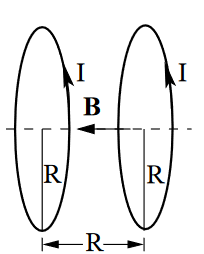
\includegraphics[width=0.5\textwidth]{content/images/KonzeptHelmholz.png}
  \caption{Schematischer Aufbau eines Helmholzspulenpaares.\cite{anleitung}.}
  \label{fig:hh}
\end{figure}

Durch die Addition der Magnetfelder beider Spulen ergibt sich
der magnetische Fluss in der Mitte eines Helmholzspulenpaares:

\begin{equation}
  B=\frac{\mu_0IR^2}{\left(R^2+x^2\right)^{3/2}}
\end{equation}

für die Änderung des magnetischen Flusses in $x$ Richtung ergibt sich daraus:

\begin{equation}
  \frac{d\,B}{d\,x}=-3\mu_0IR^2\frac{x}{\left(R^2+x^2\right)^{5/2}}
  \label{eqn:hh}
\end{equation}

Dies ist zwischen den Spulen nahezu 0, sodass sich ein nahezu konstantes Feld ergibt.

\subsection{Ferromagnet}

Ferromagnetismus ist eine erweiterte Form des Paramagnetismus.
Die geladenen Teilchen in einem Material richten sich entlang der Magnetfeldlinien
in dem Ferromagneten aus. Im Gegensatz zum Paramagneten treten die geladenen
Teilchen in dem Ferromagneten in Gruppierungen, den sogenannten weißschen Bezirken, auf und nicht einzeln auf.
Dadurch ist der Effekt der Anziehung um einiges größer als beim
Paramagnetismus. Zudem bleibt eine Restmagnetisierung, die sogenannte Remanenz.
\begin{figure}
  \centering
  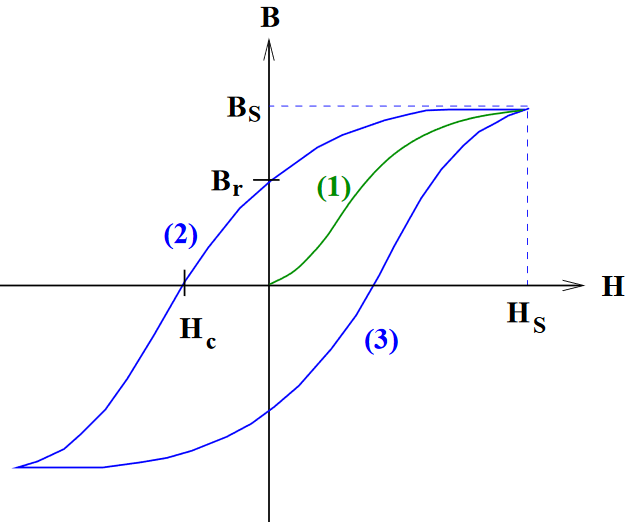
\includegraphics[width=0.5\textwidth]{content/images/Hysterese.png}
  \caption{Beispiel einer Hysteresekurve.\cite{anleitung}.}
  \label{fig:hr}
\end{figure}
Trägt man das $H$- und das $B$-Feld gegeneinander auf während
man ein Magnetfeld um den Ferromagneten auf und wieder abbaut
ergibt sich eine Hysteresekurve wie in Abb. \ref{fig:hr}. Die Nulldurchgänge
der $H$-Achse bilden die Remanenz, die der $B$-Achse bilden die Koerzität.

Formeln?
